OA\documentclass[tikz,border=5pt]{standalone}
\usepackage{amsmath}
\usepackage{tikz}
\usetikzlibrary{arrows.meta,positioning}

\begin{document}

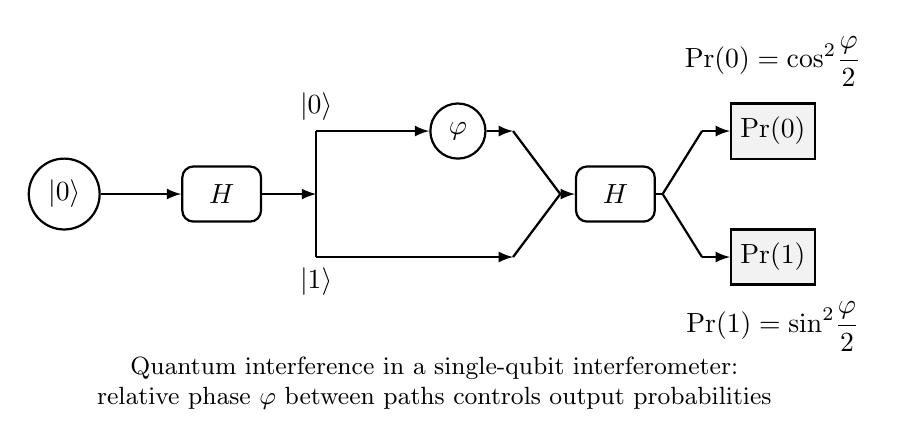
\begin{tikzpicture}[
    >=latex,
    thick,
    state/.style={circle, draw, minimum size=9mm, inner sep=0pt},
    gate/.style={rectangle, draw, rounded corners, minimum width=10mm, minimum height=7mm, align=center},
    phase/.style={circle, draw, minimum size=7mm, inner sep=0pt},
    detector/.style={rectangle, draw, minimum width=10mm, minimum height=7mm, fill=gray!10},
    label distance=3pt
]

% Horizontal positions
\def\xin{0}
\def\xHone{2.0}
\def\xsplit{3.2}
\def\xphase{5.0}
\def\xHtwo{7.0}
\def\xmeas{9.0}

% Vertical positions (paths)
\def\yupper{0.8}
\def\ylower{-0.8}

% Initial state |0>
\node[state] (psi0) at (\xin,0) {$\lvert 0\rangle$};

% First Hadamard
\node[gate] (H1) at (\xHone,0) {$H$};

% Splitting into two paths
\draw[->] (psi0) -- (H1);
\draw[->] (H1) -- (\xsplit,0);
\draw (\xsplit,0) -- (\xsplit,\yupper);
\draw (\xsplit,0) -- (\xsplit,\ylower);

% Upper path label |0>
\node[above] at (\xsplit,\yupper) {$\lvert 0\rangle$};
% Lower path label |1>
\node[below] at (\xsplit,\ylower) {$\lvert 1\rangle$};

% Phase gate on upper path
\node[phase] (P) at (\xphase,\yupper) {$\varphi$};
\draw[->] (\xsplit,\yupper) -- (P);
\draw[->] (P) -- (\xphase+0.7,\yupper);

% Lower path (no phase)
\draw[->] (\xsplit,\ylower) -- (\xphase+0.7,\ylower);

% Recombination
\draw (\xphase+0.7,\yupper) -- (\xphase+1.3,0);
\draw (\xphase+0.7,\ylower) -- (\xphase+1.3,0);

% Second Hadamard
\node[gate] (H2) at (\xHtwo,0) {$H$};
\draw[->] (\xphase+1.3,0) -- (H2);

% Measurement boxes for |0> and |1>
\node[detector] (D0) at (\xmeas,\yupper) {$\Pr(0)$};
\node[detector] (D1) at (\xmeas,\ylower) {$\Pr(1)$};

% Output split from H2 to detectors
\draw (H2.east) -- (\xHtwo+0.6,0);
\draw (\xHtwo+0.6,0) -- (\xHtwo+1.1,\yupper);
\draw (\xHtwo+0.6,0) -- (\xHtwo+1.1,\ylower);
\draw[->] (\xHtwo+1.1,\yupper) -- (D0.west);
\draw[->] (\xHtwo+1.1,\ylower) -- (D1.west);

% Interference labels
\node[above=2pt of D0.north] {$\displaystyle \Pr(0) = \cos^2\!\frac{\varphi}{2}$};
\node[below=2pt of D1.south] {$\displaystyle \Pr(1) = \sin^2\!\frac{\varphi}{2}$};

% Explanatory text
\node[align=center, font=\small] at (4.7,-2.4)
{Quantum interference in a single-qubit interferometer:\\
relative phase $\varphi$ between paths controls output probabilities};

\end{tikzpicture}
\newpage

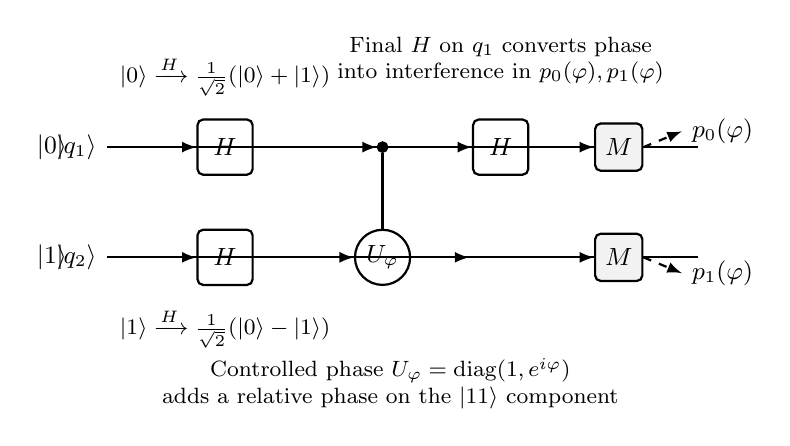
\begin{tikzpicture}[
    >=latex,
    thick,
    gate/.style={draw, rectangle, minimum width=7mm, minimum height=7mm, rounded corners=2pt},
    phasegate/.style={draw, circle, minimum size=7mm, inner sep=0pt},
    meas/.style={draw, rectangle, minimum width=6mm, minimum height=6mm, rounded corners=2pt, fill=gray!10},
    control/.style={draw, fill=black, circle, inner sep=1.2pt},
    line/.style={},
    every node/.style={font=\small}
]

% Horizontal positions
\def\xinit{0.0}
\def\xHone{1.5}
\def\xphase{3.5}
\def\xHtwo{5.0}
\def\xmeas{6.5}

% Vertical positions
\def\yqone{0.7}
\def\yqtwo{-0.7}

% Qubit labels
\node[left] at (\xinit,\yqone) {$\lvert q_1 \rangle$};
\node[left] at (\xinit,\yqtwo) {$\lvert q_2 \rangle$};

% Initial states (|0> and |1>)
\node at (\xinit-0.7,\yqone) {$\lvert 0 \rangle$};
\node at (\xinit-0.7,\yqtwo) {$\lvert 1 \rangle$};

% Wires
\draw (\xinit,\yqone) -- (\xmeas+1.0,\yqone);
\draw (\xinit,\yqtwo) -- (\xmeas+1.0,\yqtwo);

% First layer: Hadamard on both qubits
\node[gate] (H1) at (\xHone,\yqone) {$H$};
\node[gate] (H2) at (\xHone,\yqtwo) {$H$};

\draw[->] (\xinit+0.1,\yqone) -- (H1.west);
\draw[->] (\xinit+0.1,\yqtwo) -- (H2.west);

% Controlled phase U_phi on second qubit, controlled by first
\node[control] (C) at (\xphase,\yqone) {};
\node[phasegate] (P) at (\xphase,\yqtwo) {$U_\varphi$};

\draw (C) -- (P);
% input from H gates to control and target
\draw[->] (H1.east) -- (C.west);
\draw[->] (H2.east) -- (P.west);

% Second Hadamard on control qubit (to reveal interference)
\node[gate] (H3) at (\xHtwo,\yqone) {$H$};
\draw[->] (C.east) -- (H3.west);
\draw[->] (P.east) -- (\xHtwo-0.4,\yqtwo);

% Measurements
\node[meas] (M1) at (\xmeas,\yqone) {$M$};
\node[meas] (M2) at (\xmeas,\yqtwo) {$M$};

\draw[->] (H3.east) -- (M1.west);
\draw[->] (\xHtwo+0.2,\yqtwo) -- (M2.west);

% Classical readout arrows (just decorative)
\draw[->, dashed] (M1.east) -- (\xmeas+0.8,\yqone+0.2) node[right] {$p_0(\varphi)$};
\draw[->, dashed] (M2.east) -- (\xmeas+0.8,\yqtwo-0.2) node[right] {$p_1(\varphi)$};

% Annotations: superposition & phase kickback
\node[align=left, font=\footnotesize] at (1.5,1.6)
    {$\lvert 0\rangle \xrightarrow{H} \tfrac{1}{\sqrt{2}}(\lvert 0\rangle + \lvert 1\rangle)$};
\node[align=left, font=\footnotesize] at (1.5,-1.6)
    {$\lvert 1\rangle \xrightarrow{H} \tfrac{1}{\sqrt{2}}(\lvert 0\rangle - \lvert 1\rangle)$};

\node[align=center, font=\footnotesize] at (3.6,-2.3)
    {Controlled phase $U_\varphi = \mathrm{diag}(1, e^{i\varphi})$\\
     adds a relative phase on the $\lvert 11\rangle$ component};

\node[align=center, font=\footnotesize] at (5.0,1.8)
    {Final $H$ on $q_1$ converts phase\\
     into interference in $p_0(\varphi), p_1(\varphi)$};

\end{tikzpicture}

\newpage



\begin{tikzpicture}[
=latex,
   thick,
   gate/.style={draw, rectangle, minimum width=7mm, minimum height=7mm, rounded corners=2pt},
   phasegate/.style={draw, rectangle, minimum width=10mm, minimum height=7mm, rounded corners=2pt},
   meas/.style={draw, rectangle, minimum width=6mm, minimum height=6mm, rounded corners=2pt, fill=gray!10},
   control/.style={draw, fill=black, circle, inner sep=1.2pt},
   legendbox/.style={draw, rounded corners, fill=gray!5, align=center, inner sep=6pt, blur shadow},
   every node/.style={font=\small}
]

% Horizontal positions
\def\xinit{0.0}
\def\xH{1.5}
\def\xU1{3.0}
\def\xU2{4.0}
\def\xqft{5.5}
\def\xmeas{7.0}

% Vertical positions
\def\yq0{1.0}   % most significant qubit
\def\yq1{0.0}   % least significant qubit
\def\ypsi{-1.5} % target eigenstate qubit

% Qubit labels
\node[left] at (\xinit,\yq0) {$\lvert q_0 \rangle$};
\node[left] at (\xinit,\yq1) {$\lvert q_1 \rangle$};
\node[left] at (\xinit,\ypsi) {$\lvert \psi \rangle$};

% Initial states
\node at (\xinit-0.7,\yq0) {$\lvert 0 \rangle$};
\node at (\xinit-0.7,\yq1) {$\lvert 0 \rangle$};
\node at (\xinit-0.7,\ypsi) {$\lvert \psi \rangle$};

% Wires
\draw (\xinit,\yq0) -- (\xmeas+1.2,\yq0);
\draw (\xinit,\yq1) -- (\xmeas+1.2,\yq1);
\draw (\xinit,\ypsi) -- (\xmeas+1.2,\ypsi);

% Hadamards on q0 and q1
\node[gate] (H0) at (\xH,\yq0) {$H$};
\node[gate] (H1) at (\xH,\yq1) {$H$};

\draw[->] (\xinit+0.1,\yq0) -- (H0.west);
\draw[->] (\xinit+0.1,\yq1) -- (H1.west);

\draw[->] (\xinit+0.1,\ypsi) -- (\xH-0.4,\ypsi);

% Controlled-U^{2^0}
\node[control] (C1) at (\xU1,\yq1) {};
\node[phasegate] (U1) at (\xU1,\ypsi) {$U^{2^0}$};
\draw (C1) -- (U1);
\draw[->] (H1.east) -- (C1.west);
\draw[->] (\xH+0.4,\ypsi) -- (U1.west);

% Controlled-U^{2^1}
\node[control] (C0) at (\xU2,\yq0) {};
\node[phasegate] (U2) at (\xU2,\ypsi) {$U^{2^1}$};
\draw (C0) -- (U2);
\draw[->] (H0.east) -- (C0.west);
\draw[->] (U1.east) -- (\xU2-0.4,\ypsi);
\draw[->] (U2.east) -- (\xqft-0.4,\ypsi);

% Inverse QFT on q0 and q1
\node[gate] (QFT0) at (\xqft,\yq0) {$\mathrm{QFT}^{\dagger}$};
\node[gate] (QFT1) at (\xqft,\yq1) {$\mathrm{QFT}^{\dagger}$};

\draw[->] (C0.east) -- (QFT0.west);
\draw[->] (C1.east) -- (QFT1.west);

% Measurements
\node[meas] (M0) at (\xmeas,\yq0) {$M$};
\node[meas] (M1) at (\xmeas,\yq1) {$M$};

\draw[->] (QFT0.east) -- (M0.west);
\draw[->] (QFT1.east) -- (M1.west);

\draw[->, dashed] (M0.east) -- (\xmeas+1.0,\yq0+0.2) node[right] {$b_0$};
\draw[->, dashed] (M1.east) -- (\xmeas+1.0,\yq1-0.2) node[right] {$b_1$};

% --------------------------------------------------------------------
% Legend box showing state evolution (key interference formulas)
% --------------------------------------------------------------------
\node[legendbox, align=left, font=\footnotesize] (legend) at (4.0,3.2) {%
\textbf{State before inverse QFT:}\\[4pt]
$\displaystyle 
\frac{1}{2}\Big(
\lvert 00\rangle 
+ e^{2\pi i \varphi}\lvert 01\rangle 
+ e^{2\pi i 2\varphi}\lvert 10\rangle 
+ e^{2\pi i 3\varphi}\lvert 11\rangle 
\Big)$\\[6pt]
\textbf{State after inverse QFT:}\\[4pt]
$\displaystyle 
\lvert b_0 b_1\rangle \approx 
\lvert \tilde{\varphi} \rangle$\\[2pt]
$\tilde{\varphi}$ = two-bit binary approximation to $\varphi$
};

\end{tikzpicture}

\end{document}




